\section{問題定義}
\label{sec:problem_def}

本節では，バスケット構造付きトランザクションデータの形式的定義を与え，
偽共起の概念および解くべき問題を定式化する．

%% ====== 3.1 基本用語 ======
\subsection{基本用語}

\begin{definition}[アイテム・アイテムセット]
\label{def:item}
$\mathcal{I} = \{i_1, i_2, \ldots, i_m\}$ を有限のアイテム全集合とする．
$\mathcal{I}$ の任意の部分集合 $P \subseteq \mathcal{I}$ を
\emph{アイテムセット}（itemset）と呼ぶ．
$|P|$ をアイテムセット $P$ の長さとする．
\end{definition}

\begin{definition}[バスケット]
\label{def:basket}
\emph{バスケット}（basket）$B$ は，1 回の独立した購買イベントを表す
アイテムセット $B \subseteq \mathcal{I}$ である．
\end{definition}

\begin{definition}[バスケット構造付きトランザクション]
\label{def:basket_transaction}
\emph{バスケット構造付きトランザクション}（basket-structured transaction）は
タプル $d = (ts,\, \mathcal{B})$ であり，$ts \in \mathbb{Z}_{\geq 0}$ はタイムスタンプ，
$\mathcal{B} = \{B_1, B_2, \ldots, B_k\}$（$k \geq 1$）は
そのタイムスタンプに属するバスケットの集合である．
\end{definition}

\begin{definition}[バスケット構造付きトランザクションデータ]
\label{def:basket_data}
バスケット構造付きトランザクションデータ
$D = [d_1, d_2, \ldots, d_N]$ は，タイムスタンプの昇順に並べられた
バスケット構造付きトランザクションの列である．
$N = |D|$ をデータ長と呼ぶ．
\end{definition}

\noindent
\textbf{注意 (従来トランザクションとの関係)}: 定義~\ref{def:basket_transaction}において
$k = 1$，すなわち各トランザクションがちょうど 1 つのバスケットをもつ場合が
従来の頻出パターンマイニングにおけるトランザクションである．
本研究は $k \geq 1$ を許容することで，この従来設定を特殊ケースとして包含する．

%% ====== 3.2 共起の定義と偽共起 ======
\subsection{共起の定義と偽共起}

\begin{definition}[バスケット内共起（真の共起）]
\label{def:intra_basket}
トランザクション $d = (ts, \mathcal{B})$ において，アイテムセット $P$ が
\emph{バスケット内共起}（intra-basket co-occurrence）するとは，
$P$ のすべてのアイテムが \emph{同一のバスケット} $B \in \mathcal{B}$ に
含まれること，すなわち $\exists B \in \mathcal{B}: P \subseteq B$ が成立することをいう．
\end{definition}

\begin{definition}[トランザクション内共起（従来法の共起）]
\label{def:intra_transaction}
トランザクション $d = (ts, \mathcal{B})$ において，アイテムセット $P$ が
\emph{トランザクション内共起}（intra-transaction co-occurrence）するとは，
$P$ のすべてのアイテムが（バスケットを横断して）
そのトランザクションのどこかに存在すること，
すなわち $P \subseteq \bigcup_{B \in \mathcal{B}} B$ が成立することをいう．
\end{definition}

\noindent
定義~\ref{def:intra_basket} は定義~\ref{def:intra_transaction} より真に強い条件である．
すなわち，バスケット内共起 $\Rightarrow$ トランザクション内共起は常に成立するが，
逆は一般に成立しない．
異なるバスケット $B_j, B_k \in \mathcal{B}$（$j \neq k$）にそれぞれ属するアイテム同士は，
トランザクション内共起はするものの，バスケット内共起はしない．

\begin{figure}[t]
    \centering
    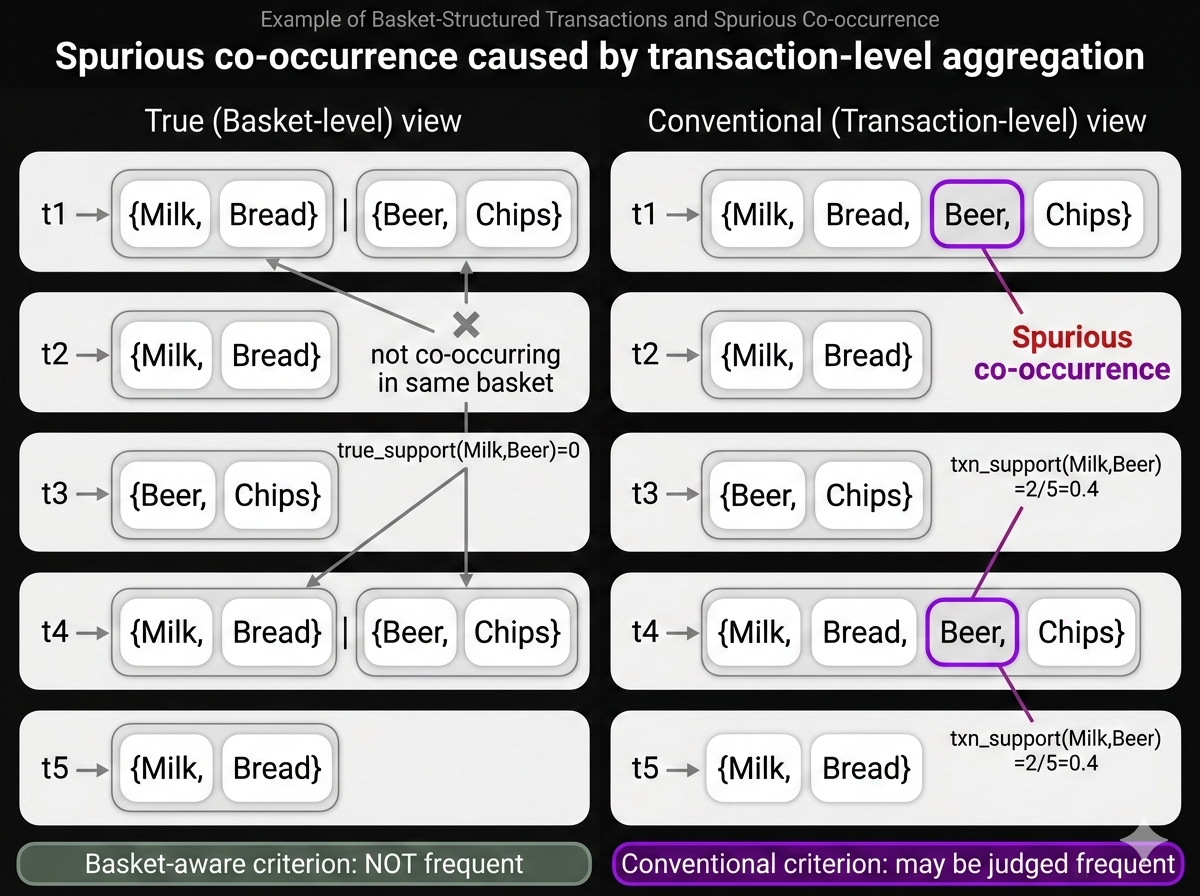
\includegraphics[width=\linewidth]{fig/example_table.png}
    \caption{バスケット構造付きトランザクションデータの例（5 トランザクション）}
    \label{fig:example_table}
\end{figure}

\begin{example}[偽共起の発生]
\label{ex:spurious}
図~\ref{fig:example_table} に示すデータを考える．
この図では，同一日に複数バスケットが存在し得る状況を表現しており，
バスケット内共起とトランザクション内共起の差が可視化されている．
5 つのトランザクション（日付）が存在し，各日に 1〜2 件のバスケットが記録される．

\begin{center}
\begin{tabular}{cll}
\toprule
$t$ & バスケット 1 & バスケット 2 \\
\midrule
1 & \{牛乳, パン\}     & \{ビール, ポテチ\} \\
2 & \{牛乳, バター\}   & — \\
3 & \{ビール, ポテチ\} & \{牛乳, チーズ\} \\
4 & \{牛乳, パン\}     & \{ビール, ポテチ\} \\
5 & \{牛乳, パン\}     & — \\
\bottomrule
\end{tabular}
\end{center}

アイテムセット $P = \{\text{牛乳, ビール}\}$ について，
$\text{txn\_support}(P) = 3/5 = 0.60$（$t = 1, 3, 4$ でトランザクション内共起），
$\text{true\_support}(P) = 0/5 = 0.00$（どのバスケットにも同時に含まれない）．

最小サポート $\theta = 0.5$ に対して，従来法（トランザクション内共起）では
$P$ を頻出パターンとして抽出するが，これは実際には存在しない共起関係である．
\end{example}

次に，区間上のサポートを定式化する．

\begin{definition}[区間とデータサブセット]
区間 $I = [ts_i, ts_j]$（$1 \leq i \leq j \leq N$）に対して，
$D_I = [d_i, d_{i+1}, \ldots, d_j]$ を区間 $I$ 内のトランザクション列とし，
$n(D_I) = j - i + 1$ をその長さとする．
\end{definition}

\begin{definition}[バスケット内サポート（true support）]
\label{def:true_support}
区間 $I$ におけるアイテムセット $P$ の \emph{バスケット内サポート}
（intra-basket support，true support）を
\begin{equation}
\text{true\_support}_I(P) =
\frac{\bigl|\bigl\{d = (ts, \mathcal{B}) \in D_I
\;\big|\; \exists B \in \mathcal{B},\; P \subseteq B\bigr\}\bigr|}{n(D_I)}
\label{eq:true_support}
\end{equation}
と定義する．
\end{definition}

\begin{definition}[トランザクション内サポート（txn support）]
\label{def:txn_support}
区間 $I$ における $P$ の \emph{トランザクション内サポート}
（intra-transaction support，txn support）を
\begin{equation}
\text{txn\_support}_I(P) =
\frac{\bigl|\bigl\{d = (ts, \mathcal{B}) \in D_I
\;\big|\; P \subseteq \textstyle\bigcup_{B \in \mathcal{B}} B\bigr\}\bigr|}{n(D_I)}
\label{eq:txn_support}
\end{equation}
と定義する．
\end{definition}

\begin{proposition}[単調性]
\label{prop:monotone}
任意のアイテムセット $P$，任意の区間 $I$，任意のトランザクションデータ $D$ に対して，
\begin{equation}
\text{true\_support}_I(P) \leq \text{txn\_support}_I(P)
\end{equation}
が成立する．
\end{proposition}

\begin{proof}
バスケット内共起は定義よりトランザクション内共起の十分条件であるため，
$P$ がバスケット内共起するトランザクションの集合は，
$P$ がトランザクション内共起するトランザクションの集合の部分集合である．
したがって，式~(\ref{eq:true_support})の分子 $\leq$ 式~(\ref{eq:txn_support})の分子
であり，命題が成立する．
\end{proof}

%% ====== 3.3 密集パターンと偽共起パターン ======
\subsection{密集パターンと偽共起パターン}

本稿では，先行研究 Apriori-window~\cite{dsaa2025} の密集パターン定義を
バスケット内サポートに基づいて再定義する．

\begin{definition}[バスケット対応密集区間・密集パターン]
\label{def:basket_dense}
最小サポートしきい値 $\theta$（$0 < \theta \leq 1$）および
最小区間長 $W$（$W \in \mathbb{Z}_{\geq 1}$）を与える．
区間 $I = [ts_i, ts_j]$（$n(D_I) \geq W$）がアイテムセット $P$ の
\emph{バスケット対応密集区間}（basket-aware dense interval）であるとは，
$\text{true\_support}_I(P) \geq \theta$ が成立することをいう．
アイテムセット $P$ がバスケット対応密集区間を少なくとも 1 つもつとき，
$P$ を \emph{バスケット対応密集パターン}（basket-aware dense pattern）と呼ぶ．
\end{definition}

\begin{definition}[偽共起パターン]
\label{def:spurious}
データ全体（$I = [ts_1, ts_N]$）におけるアイテムセット $P$ が
\emph{偽共起パターン}（spurious pattern）であるとは，
ある最小サポートしきい値 $\theta$ に対して
\begin{equation}
\text{txn\_support}(P) \geq \theta \quad \text{かつ} \quad
\text{true\_support}(P) < \theta
\end{equation}
が成立することをいう．
\end{definition}

\begin{definition}[偽共起パターン率 (SPR)]
\label{def:spr}
最小サポート $\theta$ に対して，
\emph{txn 頻出パターン}の集合を
$\mathcal{F}_{\text{txn}} = \{P \mid |P| \geq 2,\; \text{txn\_support}(P) \geq \theta\}$，
そのうち偽共起パターンの集合を
$\mathcal{F}_{\text{spur}} = \{P \in \mathcal{F}_{\text{txn}} \mid \text{true\_support}(P) < \theta\}$
と定義する．\emph{偽共起パターン率}（SPR: Spurious Pattern Rate）を
\begin{equation}
\text{SPR} = \frac{|\mathcal{F}_{\text{spur}}|}{|\mathcal{F}_{\text{txn}}|}
\label{eq:spr}
\end{equation}
と定義する．SPR = 0 は偽共起パターンが存在しないことを，
SPR = 1 は txn 頻出パターンがすべて偽共起であることを意味する．
\end{definition}

\noindent
\textbf{注記}: 式~(\ref{eq:spr}) はデータ全体のグローバルサポートに基づく定義であり，
局所密集パターンの偽共起率の評価は今後の課題とする．

%% ====== 3.4 問題の定式化 ======
\subsection{問題の定式化}

以上の定義に基づき，本稿が解く問題を次のように定式化する．

\medskip
\noindent
\textbf{問題 (Basket-aware Dense Pattern Mining)}: \\
入力として，バスケット構造付きトランザクションデータ $D$，
最小サポート $\theta$，最小区間長 $W$，最大アイテムセット長 $L$ を与える．
出力として，すべてのバスケット対応密集パターン $P$（$2 \leq |P| \leq L$）と
その密集区間の集合を網羅的に列挙する．
\medskip

\noindent
\textbf{従来法との関係}: トランザクション内サポート
（式~(\ref{eq:txn_support})）を用いた密集パターン抽出が従来法（flatten 後の
Apriori-window）に対応する．提案手法はこれをバスケット内サポート
（式~(\ref{eq:true_support})）に置き換えることで偽共起パターン（定義~\ref{def:spurious}）
を出力から完全に排除する．

\begin{proposition}[提案手法の SPR 保証]
\label{prop:spr_zero}
提案手法（Phase 1）が出力するすべての密集パターンについて，SPR = 0 が成立する．
\end{proposition}

\begin{proof}
提案手法はバスケット内サポート（$\text{true\_support}$）が $\theta$ 以上のパターンのみを
出力する．偽共起パターン（定義~\ref{def:spurious}）は
$\text{true\_support}(P) < \theta$ であるため，提案手法の出力に含まれない．
したがって，出力された txn 頻出パターンに占める偽共起パターンの割合は 0 であり，
SPR = 0 が成立する．
\end{proof}
